\documentclass[twoside]{book}

% Packages required by doxygen
\usepackage{fixltx2e}
\usepackage{calc}
\usepackage{doxygen}
\usepackage[export]{adjustbox} % also loads graphicx
\usepackage{graphicx}
\usepackage[utf8]{inputenc}
\usepackage{makeidx}
\usepackage{multicol}
\usepackage{multirow}
\PassOptionsToPackage{warn}{textcomp}
\usepackage{textcomp}
\usepackage[nointegrals]{wasysym}
\usepackage[table]{xcolor}

% NLS support packages
\usepackage[french]{babel}

% Font selection
\usepackage[T1]{fontenc}
\usepackage[scaled=.90]{helvet}
\usepackage{courier}
\usepackage{amssymb}
\usepackage{sectsty}
\renewcommand{\familydefault}{\sfdefault}
\allsectionsfont{%
  \fontseries{bc}\selectfont%
  \color{darkgray}%
}
\renewcommand{\DoxyLabelFont}{%
  \fontseries{bc}\selectfont%
  \color{darkgray}%
}
\newcommand{\+}{\discretionary{\mbox{\scriptsize$\hookleftarrow$}}{}{}}

% Page & text layout
\usepackage{geometry}
\geometry{%
  a4paper,%
  top=2.5cm,%
  bottom=2.5cm,%
  left=2.5cm,%
  right=2.5cm%
}
\tolerance=750
\hfuzz=15pt
\hbadness=750
\setlength{\emergencystretch}{15pt}
\setlength{\parindent}{0cm}
\setlength{\parskip}{3ex plus 2ex minus 2ex}
\makeatletter
\renewcommand{\paragraph}{%
  \@startsection{paragraph}{4}{0ex}{-1.0ex}{1.0ex}{%
    \normalfont\normalsize\bfseries\SS@parafont%
  }%
}
\renewcommand{\subparagraph}{%
  \@startsection{subparagraph}{5}{0ex}{-1.0ex}{1.0ex}{%
    \normalfont\normalsize\bfseries\SS@subparafont%
  }%
}
\makeatother

% Headers & footers
\usepackage{fancyhdr}
\pagestyle{fancyplain}
\fancyhead[LE]{\fancyplain{}{\bfseries\thepage}}
\fancyhead[CE]{\fancyplain{}{}}
\fancyhead[RE]{\fancyplain{}{\bfseries\leftmark}}
\fancyhead[LO]{\fancyplain{}{\bfseries\rightmark}}
\fancyhead[CO]{\fancyplain{}{}}
\fancyhead[RO]{\fancyplain{}{\bfseries\thepage}}
\fancyfoot[LE]{\fancyplain{}{}}
\fancyfoot[CE]{\fancyplain{}{}}
\fancyfoot[RE]{\fancyplain{}{\bfseries\scriptsize Généré par Doxygen }}
\fancyfoot[LO]{\fancyplain{}{\bfseries\scriptsize Généré par Doxygen }}
\fancyfoot[CO]{\fancyplain{}{}}
\fancyfoot[RO]{\fancyplain{}{}}
\renewcommand{\footrulewidth}{0.4pt}
\renewcommand{\chaptermark}[1]{%
  \markboth{#1}{}%
}
\renewcommand{\sectionmark}[1]{%
  \markright{\thesection\ #1}%
}

% Indices & bibliography
\usepackage{natbib}
\usepackage[titles]{tocloft}
\setcounter{tocdepth}{3}
\setcounter{secnumdepth}{5}
\makeindex

% Hyperlinks (required, but should be loaded last)
\usepackage{ifpdf}
\ifpdf
  \usepackage[pdftex,pagebackref=true]{hyperref}
\else
  \usepackage[ps2pdf,pagebackref=true]{hyperref}
\fi
\hypersetup{%
  colorlinks=true,%
  linkcolor=blue,%
  citecolor=blue,%
  unicode%
}

% Custom commands
\newcommand{\clearemptydoublepage}{%
  \newpage{\pagestyle{empty}\cleardoublepage}%
}

\usepackage{caption}
\captionsetup{labelsep=space,justification=centering,font={bf},singlelinecheck=off,skip=4pt,position=top}

%===== C O N T E N T S =====

\begin{document}

% Titlepage & ToC
\hypersetup{pageanchor=false,
             bookmarksnumbered=true,
             pdfencoding=unicode
            }
\pagenumbering{roman}
\begin{titlepage}
\vspace*{7cm}
\begin{center}%
{\Large « \+Era\+D\+U\+C\+Ktion » }\\
\vspace*{1cm}
{\large Généré par Doxygen 1.8.11}\\
\end{center}
\end{titlepage}
\clearemptydoublepage
\tableofcontents
\clearemptydoublepage
\pagenumbering{arabic}
\hypersetup{pageanchor=true}

%--- Begin generated contents ---
\chapter{Index des classes}
\section{Liste des classes}
Liste des classes, structures, unions et interfaces avec une brève description \+:\begin{DoxyCompactList}
\item\contentsline{section}{\hyperlink{structcanard__s}{canard\+\_\+s} \\*Etat des canards }{\pageref{structcanard__s}}{}
\item\contentsline{section}{\hyperlink{structcaract__mat__t}{caract\+\_\+mat\+\_\+t} }{\pageref{structcaract__mat__t}}{}
\item\contentsline{section}{\hyperlink{structcase__s}{case\+\_\+s} \\*Struct \hyperlink{structcase__s}{case\+\_\+s} \hyperlink{struct_8h_source}{struct.\+h} }{\pageref{structcase__s}}{}
\item\contentsline{section}{\hyperlink{structini__t}{ini\+\_\+t} }{\pageref{structini__t}}{}
\item\contentsline{section}{\hyperlink{structjoueur__s}{joueur\+\_\+s} \\*Brief information joueur }{\pageref{structjoueur__s}}{}
\item\contentsline{section}{\hyperlink{structjoueurm__s}{joueurm\+\_\+s} }{\pageref{structjoueurm__s}}{}
\item\contentsline{section}{\hyperlink{structmur__s}{mur\+\_\+s} \\*Etat du mur }{\pageref{structmur__s}}{}
\end{DoxyCompactList}

\chapter{Index des fichiers}
\section{Liste des fichiers}
Liste de tous les fichiers documentés avec une brève description \+:\begin{DoxyCompactList}
\item\contentsline{section}{\hyperlink{canard_8c}{canard.\+c} \\*Fonctions a propos du canard }{\pageref{canard_8c}}{}
\item\contentsline{section}{{\bfseries canard.\+h} }{\pageref{canard_8h}}{}
\item\contentsline{section}{\hyperlink{client__reseau_8c}{client\+\_\+reseau.\+c} \\*Fonctions propres au client }{\pageref{client__reseau_8c}}{}
\item\contentsline{section}{{\bfseries client\+\_\+reseau.\+h} }{\pageref{client__reseau_8h}}{}
\item\contentsline{section}{{\bfseries connection.\+h} }{\pageref{connection_8h}}{}
\item\contentsline{section}{\hyperlink{deplacer_8c}{deplacer.\+c} \\*Fichier contenant les fonctions de deplacement }{\pageref{deplacer_8c}}{}
\item\contentsline{section}{{\bfseries deplacer.\+h} }{\pageref{deplacer_8h}}{}
\item\contentsline{section}{{\bfseries deplacer\+\_\+multi.\+h} }{\pageref{deplacer__multi_8h}}{}
\item\contentsline{section}{{\bfseries event.\+h} }{\pageref{event_8h}}{}
\item\contentsline{section}{\hyperlink{fonction__multi__reseau_8c}{fonction\+\_\+multi\+\_\+reseau.\+c} \\*Programme qui gere tout ce qui est en rapport avec le joueur }{\pageref{fonction__multi__reseau_8c}}{}
\item\contentsline{section}{{\bfseries fonction\+\_\+multi\+\_\+reseau.\+h} }{\pageref{fonction__multi__reseau_8h}}{}
\item\contentsline{section}{{\bfseries Fonction\+\_\+\+S\+D\+L.\+h} }{\pageref{Fonction__SDL_8h}}{}
\item\contentsline{section}{{\bfseries include\+\_\+connection.\+h} }{\pageref{include__connection_8h}}{}
\item\contentsline{section}{\hyperlink{jeu__solo_8c}{jeu\+\_\+solo.\+c} \\*Programme des evenements possible sur le laby }{\pageref{jeu__solo_8c}}{}
\item\contentsline{section}{{\bfseries jeu\+\_\+solo.\+h} }{\pageref{jeu__solo_8h}}{}
\item\contentsline{section}{\hyperlink{joueur_8c}{joueur.\+c} \\*Programme qui gere tout ce qui est en rapport avec le joueur }{\pageref{joueur_8c}}{}
\item\contentsline{section}{{\bfseries joueur.\+h} }{\pageref{joueur_8h}}{}
\item\contentsline{section}{\hyperlink{labyrinthe_8c}{labyrinthe.\+c} \\*Programme comprennant la génération d\textquotesingle{}un labyrinthe }{\pageref{labyrinthe_8c}}{}
\item\contentsline{section}{{\bfseries labyrinthe.\+h} }{\pageref{labyrinthe_8h}}{}
\item\contentsline{section}{\hyperlink{main__reseau_8c}{main\+\_\+reseau.\+c} \\*Fonctions des main serveur et client pour le jeu en r�seau }{\pageref{main__reseau_8c}}{}
\item\contentsline{section}{{\bfseries main\+\_\+reseau.\+h} }{\pageref{main__reseau_8h}}{}
\item\contentsline{section}{\hyperlink{matrice_8c}{matrice.\+c} \\*Initialisation matrice }{\pageref{matrice_8c}}{}
\item\contentsline{section}{{\bfseries matrice.\+h} }{\pageref{matrice_8h}}{}
\item\contentsline{section}{\hyperlink{multijoueur_8c}{multijoueur.\+c} \\*Fonctions outils multijoueur }{\pageref{multijoueur_8c}}{}
\item\contentsline{section}{{\bfseries multijoueur.\+h} }{\pageref{multijoueur_8h}}{}
\item\contentsline{section}{{\bfseries multijoueur\+\_\+reseau.\+h} }{\pageref{multijoueur__reseau_8h}}{}
\item\contentsline{section}{{\bfseries nourriture.\+h} }{\pageref{nourriture_8h}}{}
\item\contentsline{section}{\hyperlink{outils_8c}{outils.\+c} \\*Programme comprennant les piegfes dans le laby }{\pageref{outils_8c}}{}
\item\contentsline{section}{{\bfseries outils.\+h} }{\pageref{outils_8h}}{}
\item\contentsline{section}{{\bfseries outils\+\_\+reseau.\+h} }{\pageref{outils__reseau_8h}}{}
\item\contentsline{section}{\hyperlink{piege_8c}{piege.\+c} \\*Programme comprennant les pieges dans le laby }{\pageref{piege_8c}}{}
\item\contentsline{section}{{\bfseries piege.\+h} }{\pageref{piege_8h}}{}
\item\contentsline{section}{\hyperlink{reproduction_8c}{reproduction.\+c} \\*Programme comprennant la reproduction des canards }{\pageref{reproduction_8c}}{}
\item\contentsline{section}{{\bfseries reproduction.\+h} }{\pageref{reproduction_8h}}{}
\item\contentsline{section}{{\bfseries sauvegarde.\+h} }{\pageref{sauvegarde_8h}}{}
\item\contentsline{section}{{\bfseries struct.\+h} }{\pageref{struct_8h}}{}
\end{DoxyCompactList}

\chapter{Documentation des classes}
\hypertarget{structcanard__s}{}\section{Référence de la structure canard\+\_\+s}
\label{structcanard__s}\index{canard\+\_\+s@{canard\+\_\+s}}


etat des canards  




{\ttfamily \#include $<$struct.\+h$>$}

\subsection*{Attributs publics}
\begin{DoxyCompactItemize}
\item 
int {\bfseries nourriture}\hypertarget{structcanard__s_aedc71d760126c557287c662235d6993d}{}\label{structcanard__s_aedc71d760126c557287c662235d6993d}

\item 
int {\bfseries etat}\hypertarget{structcanard__s_aa43426e9cde18de872923e47f6ec558a}{}\label{structcanard__s_aa43426e9cde18de872923e47f6ec558a}

\end{DoxyCompactItemize}


\subsection{Description détaillée}
etat des canards 

La documentation de cette structure a été générée à partir du fichier suivant \+:\begin{DoxyCompactItemize}
\item 
struct.\+h\end{DoxyCompactItemize}

\hypertarget{structcaract__mat__t}{}\section{Référence de la structure caract\+\_\+mat\+\_\+t}
\label{structcaract__mat__t}\index{caract\+\_\+mat\+\_\+t@{caract\+\_\+mat\+\_\+t}}


Graphe de collaboration de caract\+\_\+mat\+\_\+t\+:\nopagebreak
\begin{figure}[H]
\begin{center}
\leavevmode
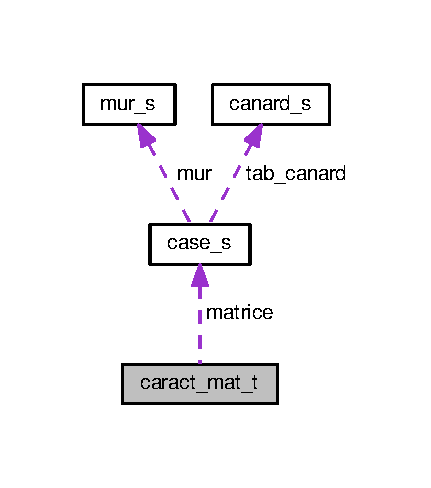
\includegraphics[width=207pt]{structcaract__mat__t__coll__graph}
\end{center}
\end{figure}
\subsection*{Attributs publics}
\begin{DoxyCompactItemize}
\item 
\hyperlink{structcase__s}{case\+\_\+t} $\ast$$\ast$ {\bfseries matrice}\hypertarget{structcaract__mat__t_aa3569a2f1b929270f199d67ba5e69e22}{}\label{structcaract__mat__t_aa3569a2f1b929270f199d67ba5e69e22}

\item 
int {\bfseries taille\+\_\+mat\+\_\+x}\hypertarget{structcaract__mat__t_a2cb8eefb38e1c69b0972af2757a56fbe}{}\label{structcaract__mat__t_a2cb8eefb38e1c69b0972af2757a56fbe}

\item 
int {\bfseries taille\+\_\+mat\+\_\+y}\hypertarget{structcaract__mat__t_a84ff012cb096bc4faf26947077ed8450}{}\label{structcaract__mat__t_a84ff012cb096bc4faf26947077ed8450}

\end{DoxyCompactItemize}


La documentation de cette structure a été générée à partir du fichier suivant \+:\begin{DoxyCompactItemize}
\item 
matrice.\+h\end{DoxyCompactItemize}

\hypertarget{structcase__s}{}\section{Référence de la structure case\+\_\+s}
\label{structcase__s}\index{case\+\_\+s@{case\+\_\+s}}


struct \hyperlink{structcase__s}{case\+\_\+s} \hyperlink{struct_8h_source}{struct.\+h}  




{\ttfamily \#include $<$struct.\+h$>$}



Graphe de collaboration de case\+\_\+s\+:\nopagebreak
\begin{figure}[H]
\begin{center}
\leavevmode
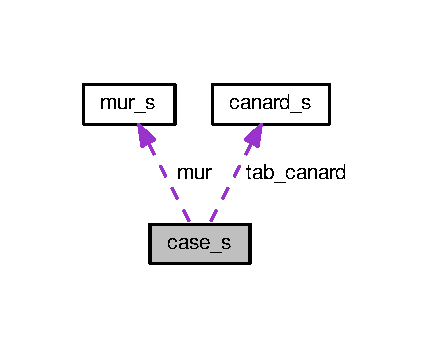
\includegraphics[width=207pt]{structcase__s__coll__graph}
\end{center}
\end{figure}
\subsection*{Attributs publics}
\begin{DoxyCompactItemize}
\item 
\hyperlink{structmur__s}{mur\+\_\+t} {\bfseries mur}\hypertarget{structcase__s_abdc07d37e4d9b61e001331ade6b389ea}{}\label{structcase__s_abdc07d37e4d9b61e001331ade6b389ea}

\item 
\hyperlink{structcanard__s}{canard\+\_\+t} {\bfseries tab\+\_\+canard} \mbox{[}nb\+\_\+max\mbox{]}\hypertarget{structcase__s_aae0820a1cce02a09249c9078bd50d4e8}{}\label{structcase__s_aae0820a1cce02a09249c9078bd50d4e8}

\item 
int {\bfseries nb\+\_\+occupant}\hypertarget{structcase__s_a3afb11c4122087e0686451fbaefebb2e}{}\label{structcase__s_a3afb11c4122087e0686451fbaefebb2e}

\item 
int {\bfseries pres\+\_\+nourriture}\hypertarget{structcase__s_a550d1707850b0078d6bad63cdce01fa3}{}\label{structcase__s_a550d1707850b0078d6bad63cdce01fa3}

\item 
int {\bfseries pres\+\_\+piege}\hypertarget{structcase__s_a8ac60b2215c63b94f4d83fd4085bbda5}{}\label{structcase__s_a8ac60b2215c63b94f4d83fd4085bbda5}

\end{DoxyCompactItemize}


\subsection{Description détaillée}
struct \hyperlink{structcase__s}{case\+\_\+s} \hyperlink{struct_8h_source}{struct.\+h} 

etat des cases 

La documentation de cette structure a été générée à partir du fichier suivant \+:\begin{DoxyCompactItemize}
\item 
struct.\+h\end{DoxyCompactItemize}

\hypertarget{structini__t}{}\section{Référence de la structure ini\+\_\+t}
\label{structini__t}\index{ini\+\_\+t@{ini\+\_\+t}}


Graphe de collaboration de ini\+\_\+t\+:\nopagebreak
\begin{figure}[H]
\begin{center}
\leavevmode
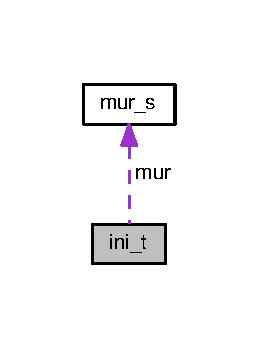
\includegraphics[width=124pt]{structini__t__coll__graph}
\end{center}
\end{figure}
\subsection*{Attributs publics}
\begin{DoxyCompactItemize}
\item 
\hyperlink{structmur__s}{mur\+\_\+t} \hyperlink{structini__t_a05761ad37f05a88ecaa33a8c380aacda}{mur}\hypertarget{structini__t_a05761ad37f05a88ecaa33a8c380aacda}{}\label{structini__t_a05761ad37f05a88ecaa33a8c380aacda}

\begin{DoxyCompactList}\small\item\em Strucure appelant une structure mur\+\_\+t, et une valeur de case. \end{DoxyCompactList}\item 
int {\bfseries valeur}\hypertarget{structini__t_a1465159977fe10d194f9117c8c664834}{}\label{structini__t_a1465159977fe10d194f9117c8c664834}

\end{DoxyCompactItemize}


La documentation de cette structure a été générée à partir du fichier suivant \+:\begin{DoxyCompactItemize}
\item 
labyrinthe.\+h\end{DoxyCompactItemize}

\hypertarget{structjoueur__s}{}\section{Référence de la structure joueur\+\_\+s}
\label{structjoueur__s}\index{joueur\+\_\+s@{joueur\+\_\+s}}


brief information joueur  




{\ttfamily \#include $<$struct.\+h$>$}

\subsection*{Attributs publics}
\begin{DoxyCompactItemize}
\item 
int {\bfseries score}\hypertarget{structjoueur__s_a403729367527db1e5b348a6e82dee49b}{}\label{structjoueur__s_a403729367527db1e5b348a6e82dee49b}

\item 
char {\bfseries nom\+\_\+joueur} \mbox{[}25\mbox{]}\hypertarget{structjoueur__s_a6bc122cdcd66bdcd44e0d774f0a6c34f}{}\label{structjoueur__s_a6bc122cdcd66bdcd44e0d774f0a6c34f}

\end{DoxyCompactItemize}


\subsection{Description détaillée}
brief information joueur 

La documentation de cette structure a été générée à partir du fichier suivant \+:\begin{DoxyCompactItemize}
\item 
struct.\+h\end{DoxyCompactItemize}

\hypertarget{structjoueurm__s}{}\section{Référence de la structure joueurm\+\_\+s}
\label{structjoueurm__s}\index{joueurm\+\_\+s@{joueurm\+\_\+s}}


Graphe de collaboration de joueurm\+\_\+s\+:\nopagebreak
\begin{figure}[H]
\begin{center}
\leavevmode
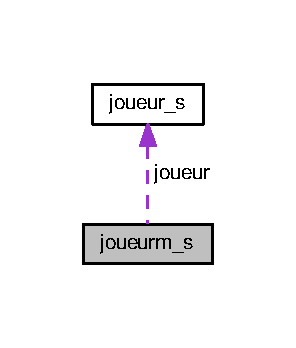
\includegraphics[width=142pt]{structjoueurm__s__coll__graph}
\end{center}
\end{figure}
\subsection*{Attributs publics}
\begin{DoxyCompactItemize}
\item 
\hyperlink{structjoueur__s}{joueur\+\_\+t} {\bfseries joueur}\hypertarget{structjoueurm__s_adb23e424b4149c57a0a67ec8cf2d9c79}{}\label{structjoueurm__s_adb23e424b4149c57a0a67ec8cf2d9c79}

\item 
clan\+\_\+t {\bfseries clan}\hypertarget{structjoueurm__s_ad121cc6e2377bdc011889472c18bc094}{}\label{structjoueurm__s_ad121cc6e2377bdc011889472c18bc094}

\item 
char {\bfseries nom} \mbox{[}20\mbox{]}\hypertarget{structjoueurm__s_afefb62cb34b9cd50ae51836fcc048e91}{}\label{structjoueurm__s_afefb62cb34b9cd50ae51836fcc048e91}

\item 
void($\ast$ {\bfseries choix} )(\hyperlink{structcaract__mat__t}{caract\+\_\+mat\+\_\+t} $\ast$, \hyperlink{structjoueur__s}{joueur\+\_\+t} $\ast$, \hyperlink{structjoueur__s}{joueur\+\_\+t} $\ast$, int $\ast$, int $\ast$, int)\hypertarget{structjoueurm__s_ac8bc4a90e2b4ae1809dd47e270bf90af}{}\label{structjoueurm__s_ac8bc4a90e2b4ae1809dd47e270bf90af}

\end{DoxyCompactItemize}


La documentation de cette structure a été générée à partir du fichier suivant \+:\begin{DoxyCompactItemize}
\item 
multijoueur.\+h\end{DoxyCompactItemize}

\hypertarget{structmur__s}{}\section{Référence de la structure mur\+\_\+s}
\label{structmur__s}\index{mur\+\_\+s@{mur\+\_\+s}}


etat du mur  




{\ttfamily \#include $<$struct.\+h$>$}

\subsection*{Attributs publics}
\begin{DoxyCompactItemize}
\item 
int {\bfseries murN}\hypertarget{structmur__s_a17fd69de75a8b0bc1975a659b235fa4a}{}\label{structmur__s_a17fd69de75a8b0bc1975a659b235fa4a}

\item 
int {\bfseries murS}\hypertarget{structmur__s_a103d980d084e67100686210daa1fa34d}{}\label{structmur__s_a103d980d084e67100686210daa1fa34d}

\item 
int {\bfseries murE}\hypertarget{structmur__s_a8c8cf029bd21f911a76a0894a61df8d6}{}\label{structmur__s_a8c8cf029bd21f911a76a0894a61df8d6}

\item 
int {\bfseries murO}\hypertarget{structmur__s_a2bd00779b370f6d650d525110c29f89b}{}\label{structmur__s_a2bd00779b370f6d650d525110c29f89b}

\end{DoxyCompactItemize}


\subsection{Description détaillée}
etat du mur 

La documentation de cette structure a été générée à partir du fichier suivant \+:\begin{DoxyCompactItemize}
\item 
struct.\+h\end{DoxyCompactItemize}

\chapter{Documentation des fichiers}
\hypertarget{canard_8c}{}\section{Référence du fichier canard.\+c}
\label{canard_8c}\index{canard.\+c@{canard.\+c}}


Fonctions outils multijoueur.  


{\ttfamily \#include $<$stdio.\+h$>$}\\*
{\ttfamily \#include $<$stdlib.\+h$>$}\\*
{\ttfamily \#include \char`\"{}struct.\+h\char`\"{}}\\*
{\ttfamily \#include \char`\"{}matrice.\+h\char`\"{}}\\*
Graphe des dépendances par inclusion de canard.\+c\+:
\nopagebreak
\begin{figure}[H]
\begin{center}
\leavevmode
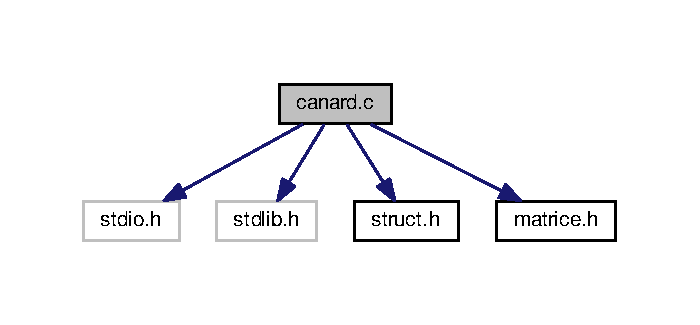
\includegraphics[width=336pt]{canard_8c__incl}
\end{center}
\end{figure}
\subsection*{Fonctions}
\begin{DoxyCompactItemize}
\item 
void \hyperlink{canard_8c_a90ecbbfe8dc92a0c4a3038a6abb20124}{init\+\_\+canard} (\hyperlink{structcaract__mat__t}{caract\+\_\+mat\+\_\+t} $\ast$cmat)
\item 
int \hyperlink{canard_8c_aa035ff52c520519ec35815a8d064f3ca}{presence\+\_\+canard} (\hyperlink{structcaract__mat__t}{caract\+\_\+mat\+\_\+t} $\ast$cmat)
\begin{DoxyCompactList}\small\item\em int \hyperlink{canard_8c_aa035ff52c520519ec35815a8d064f3ca}{presence\+\_\+canard(caract\+\_\+mat\+\_\+t $\ast$ cmat)} \end{DoxyCompactList}\item 
int \hyperlink{canard_8c_a33741fa352b02503340171e0de192c3e}{nombre\+\_\+canard} (\hyperlink{structcaract__mat__t}{caract\+\_\+mat\+\_\+t} $\ast$cmat)
\item 
int \hyperlink{canard_8c_a4716b2bc2c62ac9e65d49e81113bd511}{oeuf\+\_\+to\+\_\+adulte} (\hyperlink{structcaract__mat__t}{caract\+\_\+mat\+\_\+t} $\ast$cmat)
\end{DoxyCompactItemize}


\subsection{Description détaillée}
Fonctions outils multijoueur. 

\begin{DoxyAuthor}{Auteur}
Camille.\+V 
\end{DoxyAuthor}
\begin{DoxyVersion}{Version}
1.\+1 
\end{DoxyVersion}
\begin{DoxyDate}{Date}
20 fevrier 2018 
\end{DoxyDate}


\subsection{Documentation des fonctions}
\index{canard.\+c@{canard.\+c}!init\+\_\+canard@{init\+\_\+canard}}
\index{init\+\_\+canard@{init\+\_\+canard}!canard.\+c@{canard.\+c}}
\subsubsection[{\texorpdfstring{init\+\_\+canard(caract\+\_\+mat\+\_\+t $\ast$cmat)}{init_canard(caract_mat_t *cmat)}}]{\setlength{\rightskip}{0pt plus 5cm}void init\+\_\+canard (
\begin{DoxyParamCaption}
\item[{{\bf caract\+\_\+mat\+\_\+t} $\ast$}]{cmat}
\end{DoxyParamCaption}
)}\hypertarget{canard_8c_a90ecbbfe8dc92a0c4a3038a6abb20124}{}\label{canard_8c_a90ecbbfe8dc92a0c4a3038a6abb20124}
met des canards dans des cases aléatoire \index{canard.\+c@{canard.\+c}!nombre\+\_\+canard@{nombre\+\_\+canard}}
\index{nombre\+\_\+canard@{nombre\+\_\+canard}!canard.\+c@{canard.\+c}}
\subsubsection[{\texorpdfstring{nombre\+\_\+canard(caract\+\_\+mat\+\_\+t $\ast$cmat)}{nombre_canard(caract_mat_t *cmat)}}]{\setlength{\rightskip}{0pt plus 5cm}int nombre\+\_\+canard (
\begin{DoxyParamCaption}
\item[{{\bf caract\+\_\+mat\+\_\+t} $\ast$}]{cmat}
\end{DoxyParamCaption}
)}\hypertarget{canard_8c_a33741fa352b02503340171e0de192c3e}{}\label{canard_8c_a33741fa352b02503340171e0de192c3e}
compte les canards présents dans la matrice \index{canard.\+c@{canard.\+c}!oeuf\+\_\+to\+\_\+adulte@{oeuf\+\_\+to\+\_\+adulte}}
\index{oeuf\+\_\+to\+\_\+adulte@{oeuf\+\_\+to\+\_\+adulte}!canard.\+c@{canard.\+c}}
\subsubsection[{\texorpdfstring{oeuf\+\_\+to\+\_\+adulte(caract\+\_\+mat\+\_\+t $\ast$cmat)}{oeuf_to_adulte(caract_mat_t *cmat)}}]{\setlength{\rightskip}{0pt plus 5cm}int oeuf\+\_\+to\+\_\+adulte (
\begin{DoxyParamCaption}
\item[{{\bf caract\+\_\+mat\+\_\+t} $\ast$}]{cmat}
\end{DoxyParamCaption}
)}\hypertarget{canard_8c_a4716b2bc2c62ac9e65d49e81113bd511}{}\label{canard_8c_a4716b2bc2c62ac9e65d49e81113bd511}
change les canards à l\textquotesingle{}état d\textquotesingle{}oeuf en canards à l\textquotesingle{}état adulte \index{canard.\+c@{canard.\+c}!presence\+\_\+canard@{presence\+\_\+canard}}
\index{presence\+\_\+canard@{presence\+\_\+canard}!canard.\+c@{canard.\+c}}
\subsubsection[{\texorpdfstring{presence\+\_\+canard(caract\+\_\+mat\+\_\+t $\ast$cmat)}{presence_canard(caract_mat_t *cmat)}}]{\setlength{\rightskip}{0pt plus 5cm}int presence\+\_\+canard (
\begin{DoxyParamCaption}
\item[{{\bf caract\+\_\+mat\+\_\+t} $\ast$}]{cmat}
\end{DoxyParamCaption}
)}\hypertarget{canard_8c_aa035ff52c520519ec35815a8d064f3ca}{}\label{canard_8c_aa035ff52c520519ec35815a8d064f3ca}


int \hyperlink{canard_8c_aa035ff52c520519ec35815a8d064f3ca}{presence\+\_\+canard(caract\+\_\+mat\+\_\+t $\ast$ cmat)} 

retourne 1 si il reste des canards 
\hypertarget{deplacer_8c}{}\section{Référence du fichier deplacer.\+c}
\label{deplacer_8c}\index{deplacer.\+c@{deplacer.\+c}}


fichier contenant les fonctions de deplacement  


{\ttfamily \#include $<$stdio.\+h$>$}\\*
{\ttfamily \#include $<$stdlib.\+h$>$}\\*
{\ttfamily \#include \char`\"{}struct.\+h\char`\"{}}\\*
{\ttfamily \#include \char`\"{}matrice.\+h\char`\"{}}\\*
{\ttfamily \#include \char`\"{}deplacer\+\_\+multi.\+h\char`\"{}}\\*
{\ttfamily \#include \char`\"{}nourriture.\+h\char`\"{}}\\*
{\ttfamily \#include \char`\"{}reproduction.\+h\char`\"{}}\\*
{\ttfamily \#include \char`\"{}labyrinthe.\+h\char`\"{}}\\*
Graphe des dépendances par inclusion de deplacer.\+c\+:
\nopagebreak
\begin{figure}[H]
\begin{center}
\leavevmode
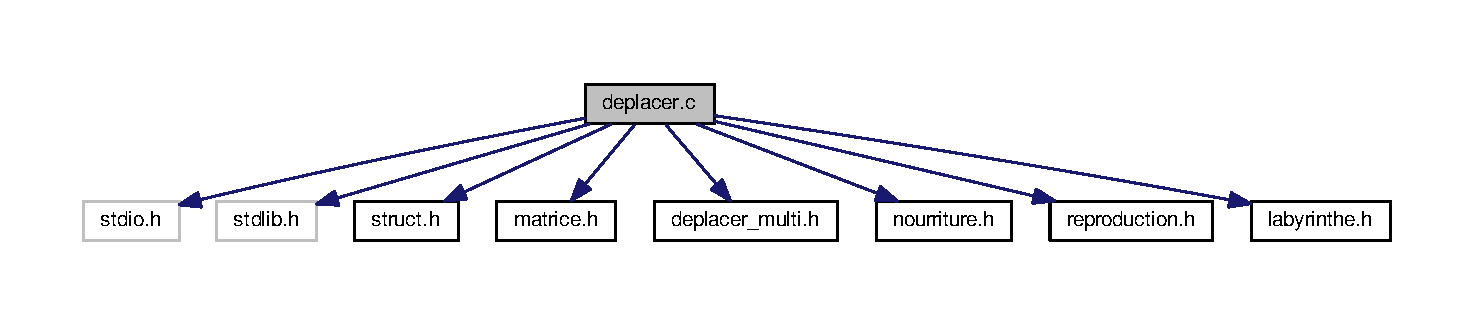
\includegraphics[width=350pt]{deplacer_8c__incl}
\end{center}
\end{figure}
\subsection*{Énumérations}
\begin{DoxyCompactItemize}
\item 
enum {\bfseries t\+\_\+direction} \{ \\*
{\bfseries Aucune\+\_\+direction} = -\/1, 
{\bfseries Est} = 1, 
{\bfseries Ouest} =2, 
{\bfseries Sud} =3, 
\\*
{\bfseries Nord} = 4, 
{\bfseries Pas\+\_\+besoin\+\_\+de\+\_\+bouger} =42
 \}\hypertarget{deplacer_8c_aec4e3894aa763e81148b2241ff730790}{}\label{deplacer_8c_aec4e3894aa763e81148b2241ff730790}

\end{DoxyCompactItemize}
\subsection*{Fonctions}
\begin{DoxyCompactItemize}
\item 
\hyperlink{structcanard__s}{canard\+\_\+t} \hyperlink{deplacer_8c_aac3daab5047434d650d678ec8422a9eb}{canard\+\_\+vide} (void)
\item 
t\+\_\+direction \hyperlink{deplacer_8c_a2e22fe142b851f5f06136b6092396121}{voit\+\_\+nourriture} (\hyperlink{structcaract__mat__t}{caract\+\_\+mat\+\_\+t} $\ast$cmat, int i, int j, int k)
\item 
t\+\_\+direction \hyperlink{deplacer_8c_aa3fbfab570f87f6a6c9ce3865f3de477}{voit\+\_\+accouplement} (\hyperlink{structcaract__mat__t}{caract\+\_\+mat\+\_\+t} $\ast$cmat, int nourriture\+\_\+accouplement, int i, int j, int kiem\+\_\+canard)
\item 
void \hyperlink{deplacer_8c_adbd99be705318964b6f5c30d9f1557c8}{deplacer\+\_\+canard} (\hyperlink{structcaract__mat__t}{caract\+\_\+mat\+\_\+t} $\ast$cmat, int i, int j, int k, int direction)
\item 
void \hyperlink{deplacer_8c_a82b2efb2b6ecb9d0e5dacddae31eb7d1}{deplacer} (\hyperlink{structcaract__mat__t}{caract\+\_\+mat\+\_\+t} $\ast$cmat, int nourriture\+\_\+accouplement, int nourriture\+\_\+genere, \hyperlink{structjoueur__s}{joueur\+\_\+t} joueur, \hyperlink{structjoueur__s}{joueur\+\_\+t} joueur2)
\end{DoxyCompactItemize}


\subsection{Description détaillée}
fichier contenant les fonctions de deplacement 

\begin{DoxyAuthor}{Auteur}
Maxime Touzé 
\end{DoxyAuthor}
\begin{DoxyVersion}{Version}
0.\+8 
\end{DoxyVersion}
\begin{DoxyDate}{Date}
19 fevrier 2018
\end{DoxyDate}
\begin{DoxyAuthor}{Auteur}
Maxime Touzé 
\end{DoxyAuthor}
\begin{DoxyVersion}{Version}
1.\+0 
\end{DoxyVersion}
\begin{DoxyDate}{Date}
19 mars 2018 
\end{DoxyDate}


\subsection{Documentation des fonctions}
\index{deplacer.\+c@{deplacer.\+c}!canard\+\_\+vide@{canard\+\_\+vide}}
\index{canard\+\_\+vide@{canard\+\_\+vide}!deplacer.\+c@{deplacer.\+c}}
\subsubsection[{\texorpdfstring{canard\+\_\+vide(void)}{canard_vide(void)}}]{\setlength{\rightskip}{0pt plus 5cm}{\bf canard\+\_\+t} canard\+\_\+vide (
\begin{DoxyParamCaption}
\item[{void}]{}
\end{DoxyParamCaption}
)}\hypertarget{deplacer_8c_aac3daab5047434d650d678ec8422a9eb}{}\label{deplacer_8c_aac3daab5047434d650d678ec8422a9eb}
renvoit un canard inexistant \index{deplacer.\+c@{deplacer.\+c}!deplacer@{deplacer}}
\index{deplacer@{deplacer}!deplacer.\+c@{deplacer.\+c}}
\subsubsection[{\texorpdfstring{deplacer(caract\+\_\+mat\+\_\+t $\ast$cmat, int nourriture\+\_\+accouplement, int nourriture\+\_\+genere, joueur\+\_\+t joueur, joueur\+\_\+t joueur2)}{deplacer(caract_mat_t *cmat, int nourriture_accouplement, int nourriture_genere, joueur_t joueur, joueur_t joueur2)}}]{\setlength{\rightskip}{0pt plus 5cm}void deplacer (
\begin{DoxyParamCaption}
\item[{{\bf caract\+\_\+mat\+\_\+t} $\ast$}]{cmat, }
\item[{int}]{nourriture\+\_\+accouplement, }
\item[{int}]{nourriture\+\_\+genere, }
\item[{{\bf joueur\+\_\+t}}]{joueur, }
\item[{{\bf joueur\+\_\+t}}]{joueur2}
\end{DoxyParamCaption}
)}\hypertarget{deplacer_8c_a82b2efb2b6ecb9d0e5dacddae31eb7d1}{}\label{deplacer_8c_a82b2efb2b6ecb9d0e5dacddae31eb7d1}
fonction qui déplace des canards tirés au sort d une case puis d une autre \index{deplacer.\+c@{deplacer.\+c}!deplacer\+\_\+canard@{deplacer\+\_\+canard}}
\index{deplacer\+\_\+canard@{deplacer\+\_\+canard}!deplacer.\+c@{deplacer.\+c}}
\subsubsection[{\texorpdfstring{deplacer\+\_\+canard(caract\+\_\+mat\+\_\+t $\ast$cmat, int i, int j, int k, int direction)}{deplacer_canard(caract_mat_t *cmat, int i, int j, int k, int direction)}}]{\setlength{\rightskip}{0pt plus 5cm}void deplacer\+\_\+canard (
\begin{DoxyParamCaption}
\item[{{\bf caract\+\_\+mat\+\_\+t} $\ast$}]{cmat, }
\item[{int}]{i, }
\item[{int}]{j, }
\item[{int}]{k, }
\item[{int}]{direction}
\end{DoxyParamCaption}
)}\hypertarget{deplacer_8c_adbd99be705318964b6f5c30d9f1557c8}{}\label{deplacer_8c_adbd99be705318964b6f5c30d9f1557c8}
Deplace le kieme canard de la case i;j dans la direction donnée \index{deplacer.\+c@{deplacer.\+c}!voit\+\_\+accouplement@{voit\+\_\+accouplement}}
\index{voit\+\_\+accouplement@{voit\+\_\+accouplement}!deplacer.\+c@{deplacer.\+c}}
\subsubsection[{\texorpdfstring{voit\+\_\+accouplement(caract\+\_\+mat\+\_\+t $\ast$cmat, int nourriture\+\_\+accouplement, int i, int j, int kiem\+\_\+canard)}{voit_accouplement(caract_mat_t *cmat, int nourriture_accouplement, int i, int j, int kiem_canard)}}]{\setlength{\rightskip}{0pt plus 5cm}t\+\_\+direction voit\+\_\+accouplement (
\begin{DoxyParamCaption}
\item[{{\bf caract\+\_\+mat\+\_\+t} $\ast$}]{cmat, }
\item[{int}]{nourriture\+\_\+accouplement, }
\item[{int}]{i, }
\item[{int}]{j, }
\item[{int}]{kiem\+\_\+canard}
\end{DoxyParamCaption}
)}\hypertarget{deplacer_8c_aa3fbfab570f87f6a6c9ce3865f3de477}{}\label{deplacer_8c_aa3fbfab570f87f6a6c9ce3865f3de477}
fonction qui renvoit la direction dans laquelle le canard k de la case i;j voit un partenaire de reprod (-\/1 si pas de vision dessus)

SI pas de mur enregistré on regarde si il y a un partenaire d accouplement, si c est le cas on break, puis on regarde si il y a un mur, et si il y a on memorise qu il y en a un et on verifie que tous les murs soient pas trouvés\index{deplacer.\+c@{deplacer.\+c}!voit\+\_\+nourriture@{voit\+\_\+nourriture}}
\index{voit\+\_\+nourriture@{voit\+\_\+nourriture}!deplacer.\+c@{deplacer.\+c}}
\subsubsection[{\texorpdfstring{voit\+\_\+nourriture(caract\+\_\+mat\+\_\+t $\ast$cmat, int i, int j, int k)}{voit_nourriture(caract_mat_t *cmat, int i, int j, int k)}}]{\setlength{\rightskip}{0pt plus 5cm}t\+\_\+direction voit\+\_\+nourriture (
\begin{DoxyParamCaption}
\item[{{\bf caract\+\_\+mat\+\_\+t} $\ast$}]{cmat, }
\item[{int}]{i, }
\item[{int}]{j, }
\item[{int}]{k}
\end{DoxyParamCaption}
)}\hypertarget{deplacer_8c_a2e22fe142b851f5f06136b6092396121}{}\label{deplacer_8c_a2e22fe142b851f5f06136b6092396121}
fonction qui renvoit la direction dans laquelle le canard k de la case i;j voit de la nouriture (-\/1 si pas de vision dessus)

SI pas de mur enregistré on regarde si il y a un fruit, si c est le cas on break, puis on regarde si il y a un mur, et si il y a on memorise qu il y en a un et on verifie que tous les murs soient pas trouvés
\hypertarget{jeu__solo_8c}{}\section{Référence du fichier jeu\+\_\+solo.\+c}
\label{jeu__solo_8c}\index{jeu\+\_\+solo.\+c@{jeu\+\_\+solo.\+c}}


programme des evenements possible sur le laby  


{\ttfamily \#include $<$stdio.\+h$>$}\\*
{\ttfamily \#include \char`\"{}struct.\+h\char`\"{}}\\*
{\ttfamily \#include \char`\"{}matrice.\+h\char`\"{}}\\*
{\ttfamily \#include \char`\"{}piege.\+h\char`\"{}}\\*
{\ttfamily \#include \char`\"{}nourriture.\+h\char`\"{}}\\*
{\ttfamily \#include \char`\"{}joueur.\+h\char`\"{}}\\*
{\ttfamily \#include \char`\"{}canard.\+h\char`\"{}}\\*
{\ttfamily \#include \char`\"{}deplacer.\+h\char`\"{}}\\*
{\ttfamily \#include \char`\"{}deplacer\+\_\+multi.\+h\char`\"{}}\\*
{\ttfamily \#include \char`\"{}labyrinthe.\+h\char`\"{}}\\*
Graphe des dépendances par inclusion de jeu\+\_\+solo.\+c\+:\nopagebreak
\begin{figure}[H]
\begin{center}
\leavevmode
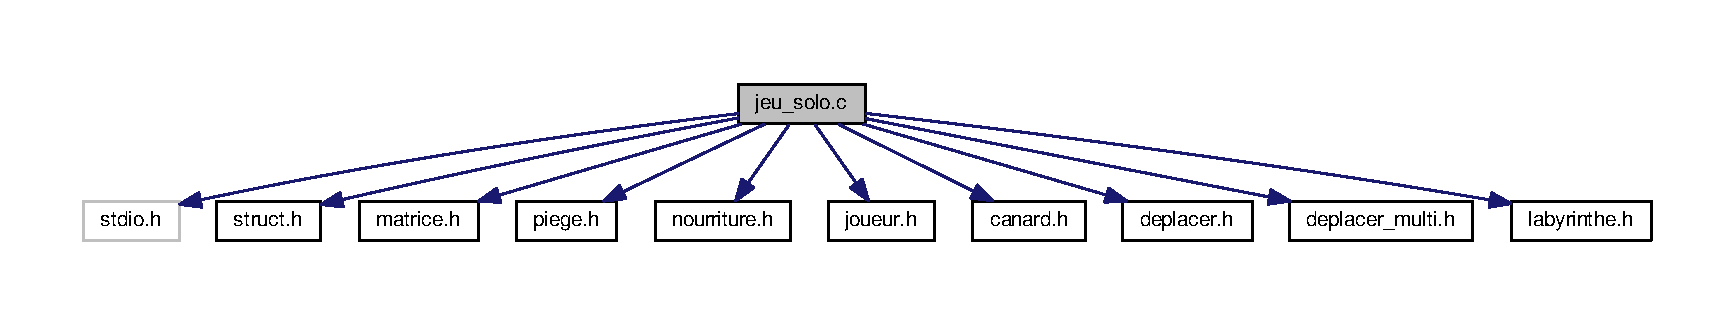
\includegraphics[width=350pt]{jeu__solo_8c__incl}
\end{center}
\end{figure}
\subsection*{Fonctions}
\begin{DoxyCompactItemize}
\item 
int \hyperlink{jeu__solo_8c_a293021ac3e183901d8afa48b6575f425}{jeu\+\_\+solo} (\hyperlink{structcaract__mat__t}{caract\+\_\+mat\+\_\+t} $\ast$cmat, int nourriture\+\_\+genere, int nourriture\+\_\+accouplement, \hyperlink{structjoueur__s}{joueur\+\_\+t} $\ast$joueur, \hyperlink{structjoueur__s}{joueur\+\_\+t} $\ast$joueur2, int nb\+\_\+gen)\hypertarget{jeu__solo_8c_a293021ac3e183901d8afa48b6575f425}{}\label{jeu__solo_8c_a293021ac3e183901d8afa48b6575f425}

\begin{DoxyCompactList}\small\item\em fonction qui fait le déroulement du jeu \end{DoxyCompactList}\end{DoxyCompactItemize}


\subsection{Description détaillée}
programme des evenements possible sur le laby 

Algo de jeu solo.

\begin{DoxyAuthor}{Auteur}
P\+H\+I\+L\+L\+I\+PE Marion 
\end{DoxyAuthor}
\begin{DoxyVersion}{Version}
1.\+0 
\end{DoxyVersion}
\begin{DoxyDate}{Date}
19 Mars 2018
\end{DoxyDate}
\begin{DoxyAuthor}{Auteur}
P\+H\+I\+L\+L\+I\+PE Marion 
\end{DoxyAuthor}
\begin{DoxyVersion}{Version}
1.\+1 
\end{DoxyVersion}
\begin{DoxyDate}{Date}
19 Mars 2018 
\end{DoxyDate}

\hypertarget{joueur_8c}{}\section{Référence du fichier joueur.\+c}
\label{joueur_8c}\index{joueur.\+c@{joueur.\+c}}


programme qui gere tout ce qui est en rapport avec le joueur  


{\ttfamily \#include $<$stdio.\+h$>$}\\*
{\ttfamily \#include $<$stdlib.\+h$>$}\\*
{\ttfamily \#include \char`\"{}struct.\+h\char`\"{}}\\*
{\ttfamily \#include \char`\"{}matrice.\+h\char`\"{}}\\*
{\ttfamily \#include \char`\"{}event.\+h\char`\"{}}\\*
{\ttfamily \#include \char`\"{}string.\+h\char`\"{}}\\*
Graphe des dépendances par inclusion de joueur.\+c\+:
\nopagebreak
\begin{figure}[H]
\begin{center}
\leavevmode
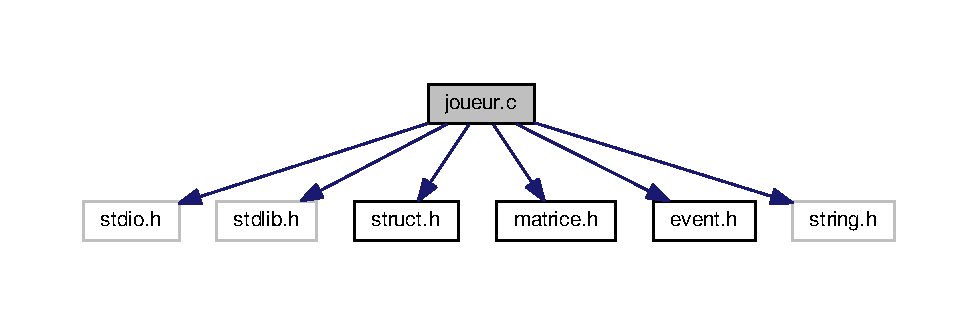
\includegraphics[width=350pt]{joueur_8c__incl}
\end{center}
\end{figure}
\subsection*{Macros}
\begin{DoxyCompactItemize}
\item 
\#define {\bfseries nb\+\_\+event}~5\hypertarget{joueur_8c_a7dfdd4832588adc97043924fb55d4bd5}{}\label{joueur_8c_a7dfdd4832588adc97043924fb55d4bd5}

\end{DoxyCompactItemize}
\subsection*{Fonctions}
\begin{DoxyCompactItemize}
\item 
void \hyperlink{joueur_8c_ac66b42d166b322e1db00bd2177764549}{ajout\+\_\+score} (int point, \hyperlink{structjoueur__s}{joueur\+\_\+t} $\ast$joueur, \hyperlink{structjoueur__s}{joueur\+\_\+t} $\ast$joueur2)
\item 
void \hyperlink{joueur_8c_a72017265abfb242c8d9c99dd1531a978}{caract\+\_\+joueur} (\hyperlink{structjoueur__s}{joueur\+\_\+t} $\ast$joueur)
\item 
void \hyperlink{joueur_8c_ac45960f5f46db2ff59140d731408b4a3}{tab\+\_\+event\+\_\+mauvais} (int $\ast$choix1, int $\ast$choix2, int $\ast$choix3)\hypertarget{joueur_8c_ac45960f5f46db2ff59140d731408b4a3}{}\label{joueur_8c_ac45960f5f46db2ff59140d731408b4a3}

\begin{DoxyCompactList}\small\item\em choisit 3 mauvais evenements random \end{DoxyCompactList}\item 
void \hyperlink{joueur_8c_a78c07d9604fba01b03805482806cb0e2}{tab\+\_\+event\+\_\+bon} (int $\ast$choix1, int $\ast$choix2, int $\ast$choix3)\hypertarget{joueur_8c_a78c07d9604fba01b03805482806cb0e2}{}\label{joueur_8c_a78c07d9604fba01b03805482806cb0e2}

\begin{DoxyCompactList}\small\item\em choisit 3 bons evenements random \end{DoxyCompactList}\item 
void \hyperlink{joueur_8c_a21f905f6f541961cde54b018f809411b}{choix\+\_\+mechant} (\hyperlink{structcaract__mat__t}{caract\+\_\+mat\+\_\+t} $\ast$cmat, \hyperlink{structjoueur__s}{joueur\+\_\+t} joueur, \hyperlink{structjoueur__s}{joueur\+\_\+t} joueur2, int $\ast$nourriture\+\_\+genere, int $\ast$nourriture\+\_\+accouplement)\hypertarget{joueur_8c_a21f905f6f541961cde54b018f809411b}{}\label{joueur_8c_a21f905f6f541961cde54b018f809411b}

\begin{DoxyCompactList}\small\item\em choix random parmis les evenements mauvais \end{DoxyCompactList}\item 
void \hyperlink{joueur_8c_adb1f4df3ebe94410f2c0bb0b1d43bdfa}{choix\+\_\+bon} (\hyperlink{structcaract__mat__t}{caract\+\_\+mat\+\_\+t} $\ast$cmat, \hyperlink{structjoueur__s}{joueur\+\_\+t} joueur, \hyperlink{structjoueur__s}{joueur\+\_\+t} joueur2, int $\ast$nourriture\+\_\+genere, int $\ast$nourriture\+\_\+accouplement)\hypertarget{joueur_8c_adb1f4df3ebe94410f2c0bb0b1d43bdfa}{}\label{joueur_8c_adb1f4df3ebe94410f2c0bb0b1d43bdfa}

\begin{DoxyCompactList}\small\item\em choix random parmis les evenements bon \end{DoxyCompactList}\item 
void \hyperlink{joueur_8c_a7032945ab7c4c1e6f628de8ec013596e}{choix\+\_\+joueur} (\hyperlink{structcaract__mat__t}{caract\+\_\+mat\+\_\+t} $\ast$cmat, \hyperlink{structjoueur__s}{joueur\+\_\+t} joueur, \hyperlink{structjoueur__s}{joueur\+\_\+t} joueur2, int $\ast$nourriture\+\_\+genere, int $\ast$nourriture\+\_\+accouplement)\hypertarget{joueur_8c_a7032945ab7c4c1e6f628de8ec013596e}{}\label{joueur_8c_a7032945ab7c4c1e6f628de8ec013596e}

\begin{DoxyCompactList}\small\item\em choix du joueur parmis les evenements \end{DoxyCompactList}\end{DoxyCompactItemize}
\subsection*{Variables}
\begin{DoxyCompactItemize}
\item 
char $\ast$ {\bfseries mauv\+\_\+evts} \mbox{[}nb\+\_\+event\mbox{]}
\item 
char $\ast$ {\bfseries bon\+\_\+evts} \mbox{[}nb\+\_\+event\mbox{]}
\end{DoxyCompactItemize}


\subsection{Description détaillée}
programme qui gere tout ce qui est en rapport avec le joueur 

\begin{DoxyAuthor}{Auteur}
V\+A\+I\+D\+IE Camille 
\end{DoxyAuthor}
\begin{DoxyVersion}{Version}
1.\+0 
\end{DoxyVersion}
\begin{DoxyDate}{Date}
20 fevrier 2018 
\end{DoxyDate}


\subsection{Documentation des fonctions}
\index{joueur.\+c@{joueur.\+c}!ajout\+\_\+score@{ajout\+\_\+score}}
\index{ajout\+\_\+score@{ajout\+\_\+score}!joueur.\+c@{joueur.\+c}}
\subsubsection[{\texorpdfstring{ajout\+\_\+score(int point, joueur\+\_\+t $\ast$joueur, joueur\+\_\+t $\ast$joueur2)}{ajout_score(int point, joueur_t *joueur, joueur_t *joueur2)}}]{\setlength{\rightskip}{0pt plus 5cm}void ajout\+\_\+score (
\begin{DoxyParamCaption}
\item[{int}]{point, }
\item[{{\bf joueur\+\_\+t} $\ast$}]{joueur, }
\item[{{\bf joueur\+\_\+t} $\ast$}]{joueur2}
\end{DoxyParamCaption}
)}\hypertarget{joueur_8c_ac66b42d166b322e1db00bd2177764549}{}\label{joueur_8c_ac66b42d166b322e1db00bd2177764549}
fonction d\textquotesingle{}ajour de score des deux joueurs \index{joueur.\+c@{joueur.\+c}!caract\+\_\+joueur@{caract\+\_\+joueur}}
\index{caract\+\_\+joueur@{caract\+\_\+joueur}!joueur.\+c@{joueur.\+c}}
\subsubsection[{\texorpdfstring{caract\+\_\+joueur(joueur\+\_\+t $\ast$joueur)}{caract_joueur(joueur_t *joueur)}}]{\setlength{\rightskip}{0pt plus 5cm}void caract\+\_\+joueur (
\begin{DoxyParamCaption}
\item[{{\bf joueur\+\_\+t} $\ast$}]{joueur}
\end{DoxyParamCaption}
)}\hypertarget{joueur_8c_a72017265abfb242c8d9c99dd1531a978}{}\label{joueur_8c_a72017265abfb242c8d9c99dd1531a978}
saisi du pseudo du joueur 

\subsection{Documentation des variables}
\index{joueur.\+c@{joueur.\+c}!bon\+\_\+evts@{bon\+\_\+evts}}
\index{bon\+\_\+evts@{bon\+\_\+evts}!joueur.\+c@{joueur.\+c}}
\subsubsection[{\texorpdfstring{bon\+\_\+evts}{bon_evts}}]{\setlength{\rightskip}{0pt plus 5cm}char$\ast$ bon\+\_\+evts\mbox{[}nb\+\_\+event\mbox{]}}\hypertarget{joueur_8c_af6bfe6ae8650a2efeff482531b54ec37}{}\label{joueur_8c_af6bfe6ae8650a2efeff482531b54ec37}
{\bfseries Valeur initiale \+:}
\begin{DoxyCode}
=\{
    \textcolor{stringliteral}{"Accelère la reproduction des canards"},
    \textcolor{stringliteral}{"Génération de nourriture augmentée"},
    \textcolor{stringliteral}{"Rien changer"},
    \textcolor{stringliteral}{"Libère entre 0 et 5 canards"},
    \textcolor{stringliteral}{"Rend un canard invincible"}\}
\end{DoxyCode}
\index{joueur.\+c@{joueur.\+c}!mauv\+\_\+evts@{mauv\+\_\+evts}}
\index{mauv\+\_\+evts@{mauv\+\_\+evts}!joueur.\+c@{joueur.\+c}}
\subsubsection[{\texorpdfstring{mauv\+\_\+evts}{mauv_evts}}]{\setlength{\rightskip}{0pt plus 5cm}char$\ast$ mauv\+\_\+evts\mbox{[}nb\+\_\+event\mbox{]}}\hypertarget{joueur_8c_a2853cc8ef23ae8fe1b7679e4e938de06}{}\label{joueur_8c_a2853cc8ef23ae8fe1b7679e4e938de06}
{\bfseries Valeur initiale \+:}
\begin{DoxyCode}
=\{
    \textcolor{stringliteral}{"Lance un tsunami sur le labyrinthe"}, 
    \textcolor{stringliteral}{"Lance une tempete sur le labyrinthe"},
    \textcolor{stringliteral}{"Famine : Réduit la nourriture générée"},
    \textcolor{stringliteral}{"Réduit la reproduction des canards"},
    \textcolor{stringliteral}{"Appartion de 0 à 5 prédateurs de canards"}
\}
\end{DoxyCode}

\hypertarget{labyrinthe_8c}{}\section{Référence du fichier labyrinthe.\+c}
\label{labyrinthe_8c}\index{labyrinthe.\+c@{labyrinthe.\+c}}


Programme comprennant la génération d\textquotesingle{}un labyrinthe.  


{\ttfamily \#include $<$stdio.\+h$>$}\\*
{\ttfamily \#include $<$stdlib.\+h$>$}\\*
{\ttfamily \#include $<$time.\+h$>$}\\*
{\ttfamily \#include \char`\"{}struct.\+h\char`\"{}}\\*
{\ttfamily \#include \char`\"{}matrice.\+h\char`\"{}}\\*
{\ttfamily \#include \char`\"{}labyrinthe.\+h\char`\"{}}\\*
Graphe des dépendances par inclusion de labyrinthe.\+c\+:
\nopagebreak
\begin{figure}[H]
\begin{center}
\leavevmode
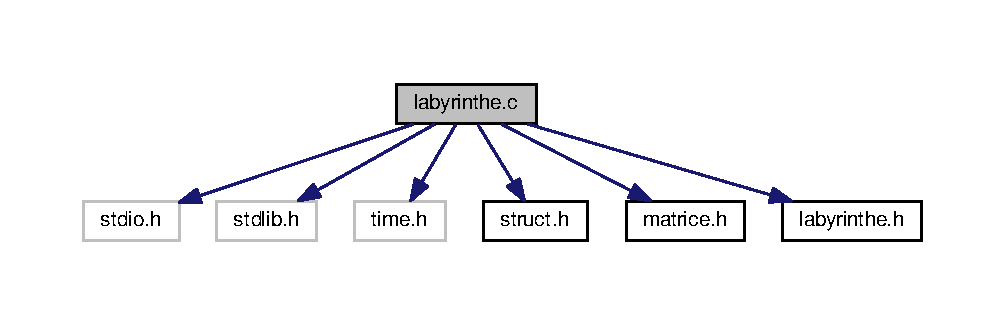
\includegraphics[width=350pt]{labyrinthe_8c__incl}
\end{center}
\end{figure}
\subsection*{Macros}
\begin{DoxyCompactItemize}
\item 
\#define {\bfseries M\+AX}~4\hypertarget{labyrinthe_8c_a392fb874e547e582e9c66a08a1f23326}{}\label{labyrinthe_8c_a392fb874e547e582e9c66a08a1f23326}

\end{DoxyCompactItemize}
\subsection*{Fonctions}
\begin{DoxyCompactItemize}
\item 
int {\bfseries compter\+\_\+murs} (\hyperlink{structcaract__mat__t}{caract\+\_\+mat\+\_\+t} $\ast$cmat, int i, int j)\hypertarget{labyrinthe_8c_aaa99616442fe50bed154bc9a599217eb}{}\label{labyrinthe_8c_aaa99616442fe50bed154bc9a599217eb}

\item 
void {\bfseries afficher\+\_\+angle} (\hyperlink{structcaract__mat__t}{caract\+\_\+mat\+\_\+t} $\ast$cmat, int j, int i)\hypertarget{labyrinthe_8c_a629d2a355cb4d64f221c3c4ed31de155}{}\label{labyrinthe_8c_a629d2a355cb4d64f221c3c4ed31de155}

\item 
void \hyperlink{labyrinthe_8c_aad84aaf14c03fe3e6c3b4378500d9530}{affichage\+\_\+laby} (\hyperlink{structcaract__mat__t}{caract\+\_\+mat\+\_\+t} $\ast$cmat)
\item 
void \hyperlink{labyrinthe_8c_a9fe6a8b9d6a89085ba3f519da212c069}{init\+\_\+laby} (\hyperlink{structcaract__mat__t}{caract\+\_\+mat\+\_\+t} $\ast$cmat, \hyperlink{structini__t}{ini\+\_\+t} $\ast$$\ast$mat)
\item 
void \hyperlink{labyrinthe_8c_ac0c9636ef89db9e46a0cf9c5fe5f3d53}{maxmin} (\hyperlink{structini__t}{ini\+\_\+t} $\ast$$\ast$mat, int $\ast$max, int $\ast$min, int val1, int val2)
\item 
void \hyperlink{labyrinthe_8c_afa2b95a96ad18258e75b6e8018a841d1}{valeur\+\_\+case} (\hyperlink{structcaract__mat__t}{caract\+\_\+mat\+\_\+t} $\ast$cmat, \hyperlink{structini__t}{ini\+\_\+t} $\ast$$\ast$mat, int x1, int y1, int x2, int y2, int $\ast$compteur)
\item 
int {\bfseries compter\+\_\+mur} (\hyperlink{structini__t}{ini\+\_\+t} $\ast$$\ast$mat, int i, int j)\hypertarget{labyrinthe_8c_a57ff2e46587e5aa49c066d614c305d25}{}\label{labyrinthe_8c_a57ff2e46587e5aa49c066d614c305d25}

\item 
void \hyperlink{labyrinthe_8c_abacc944c4e85f29e9da1dfbc2dbc0565}{case\+\_\+adja} (\hyperlink{structcaract__mat__t}{caract\+\_\+mat\+\_\+t} $\ast$cmat, \hyperlink{structini__t}{ini\+\_\+t} $\ast$$\ast$mat, int coord\+\_\+x, int coord\+\_\+y, int $\ast$compteur)
\item 
void \hyperlink{labyrinthe_8c_a97c8cd519ab9fe6f41571f8d77cfebce}{coord\+\_\+case} (\hyperlink{structcaract__mat__t}{caract\+\_\+mat\+\_\+t} $\ast$cmat, \hyperlink{structini__t}{ini\+\_\+t} $\ast$$\ast$mat, int $\ast$compteur)
\item 
int \hyperlink{labyrinthe_8c_a9ffd1e3cafcf0e3e95937442ca25b0cf}{laby\+\_\+fini} (\hyperlink{structcaract__mat__t}{caract\+\_\+mat\+\_\+t} $\ast$cmat, \hyperlink{structini__t}{ini\+\_\+t} $\ast$$\ast$mat)
\item 
void {\bfseries maj\+\_\+coins} (\hyperlink{structcaract__mat__t}{caract\+\_\+mat\+\_\+t} $\ast$cmat, \hyperlink{structini__t}{ini\+\_\+t} $\ast$$\ast$mat, int $\ast$compteur)\hypertarget{labyrinthe_8c_a30bd835edc9fd3791e437a845aae9e10}{}\label{labyrinthe_8c_a30bd835edc9fd3791e437a845aae9e10}

\item 
void \hyperlink{labyrinthe_8c_a2de2986c76d981e88d26e402eb491010}{balayage} (\hyperlink{structcaract__mat__t}{caract\+\_\+mat\+\_\+t} $\ast$cmat, \hyperlink{structini__t}{ini\+\_\+t} $\ast$$\ast$mat, int $\ast$compteur)
\item 
void \hyperlink{labyrinthe_8c_a9c756383ac514e4057850665d5b510a2}{creer\+\_\+labyrinthe} (\hyperlink{structcaract__mat__t}{caract\+\_\+mat\+\_\+t} $\ast$cmat, \hyperlink{structini__t}{ini\+\_\+t} $\ast$$\ast$mat)
\item 
void {\bfseries copi\+\_\+laby} (\hyperlink{structini__t}{ini\+\_\+t} $\ast$$\ast$mat, \hyperlink{structcaract__mat__t}{caract\+\_\+mat\+\_\+t} $\ast$cmat)\hypertarget{labyrinthe_8c_aef2db2cfc24bd4bd6bc91ccb74a0f987}{}\label{labyrinthe_8c_aef2db2cfc24bd4bd6bc91ccb74a0f987}

\item 
int {\bfseries main\+\_\+laby} (\hyperlink{structcaract__mat__t}{caract\+\_\+mat\+\_\+t} $\ast$cmat)\hypertarget{labyrinthe_8c_a1234917404dc6a2d930a06e7cff58d19}{}\label{labyrinthe_8c_a1234917404dc6a2d930a06e7cff58d19}

\end{DoxyCompactItemize}


\subsection{Description détaillée}
Programme comprennant la génération d\textquotesingle{}un labyrinthe. 

\begin{DoxyAuthor}{Auteur}
Marchand Killian Touzé Maxime 
\end{DoxyAuthor}
\begin{DoxyVersion}{Version}
3.\+0 
\end{DoxyVersion}
\begin{DoxyDate}{Date}
20 Février 2018 
\end{DoxyDate}


\subsection{Documentation des fonctions}
\index{labyrinthe.\+c@{labyrinthe.\+c}!affichage\+\_\+laby@{affichage\+\_\+laby}}
\index{affichage\+\_\+laby@{affichage\+\_\+laby}!labyrinthe.\+c@{labyrinthe.\+c}}
\subsubsection[{\texorpdfstring{affichage\+\_\+laby(caract\+\_\+mat\+\_\+t $\ast$cmat)}{affichage_laby(caract_mat_t *cmat)}}]{\setlength{\rightskip}{0pt plus 5cm}void affichage\+\_\+laby (
\begin{DoxyParamCaption}
\item[{{\bf caract\+\_\+mat\+\_\+t} $\ast$}]{cmat}
\end{DoxyParamCaption}
)}\hypertarget{labyrinthe_8c_aad84aaf14c03fe3e6c3b4378500d9530}{}\label{labyrinthe_8c_aad84aaf14c03fe3e6c3b4378500d9530}
Affichage du labyrinthe avec les murs sour forme A\+S\+C\+II \index{labyrinthe.\+c@{labyrinthe.\+c}!balayage@{balayage}}
\index{balayage@{balayage}!labyrinthe.\+c@{labyrinthe.\+c}}
\subsubsection[{\texorpdfstring{balayage(caract\+\_\+mat\+\_\+t $\ast$cmat, ini\+\_\+t $\ast$$\ast$mat, int $\ast$compteur)}{balayage(caract_mat_t *cmat, ini_t **mat, int *compteur)}}]{\setlength{\rightskip}{0pt plus 5cm}void balayage (
\begin{DoxyParamCaption}
\item[{{\bf caract\+\_\+mat\+\_\+t} $\ast$}]{cmat, }
\item[{{\bf ini\+\_\+t} $\ast$$\ast$}]{mat, }
\item[{int $\ast$}]{compteur}
\end{DoxyParamCaption}
)}\hypertarget{labyrinthe_8c_a2de2986c76d981e88d26e402eb491010}{}\label{labyrinthe_8c_a2de2986c76d981e88d26e402eb491010}
foncion qui parcoure la matrice et si il y a deux cases adjacentes qui ont une valeur différente elle casse le mur entre les deux \index{labyrinthe.\+c@{labyrinthe.\+c}!case\+\_\+adja@{case\+\_\+adja}}
\index{case\+\_\+adja@{case\+\_\+adja}!labyrinthe.\+c@{labyrinthe.\+c}}
\subsubsection[{\texorpdfstring{case\+\_\+adja(caract\+\_\+mat\+\_\+t $\ast$cmat, ini\+\_\+t $\ast$$\ast$mat, int coord\+\_\+x, int coord\+\_\+y, int $\ast$compteur)}{case_adja(caract_mat_t *cmat, ini_t **mat, int coord_x, int coord_y, int *compteur)}}]{\setlength{\rightskip}{0pt plus 5cm}void case\+\_\+adja (
\begin{DoxyParamCaption}
\item[{{\bf caract\+\_\+mat\+\_\+t} $\ast$}]{cmat, }
\item[{{\bf ini\+\_\+t} $\ast$$\ast$}]{mat, }
\item[{int}]{coord\+\_\+x, }
\item[{int}]{coord\+\_\+y, }
\item[{int $\ast$}]{compteur}
\end{DoxyParamCaption}
)}\hypertarget{labyrinthe_8c_abacc944c4e85f29e9da1dfbc2dbc0565}{}\label{labyrinthe_8c_abacc944c4e85f29e9da1dfbc2dbc0565}
Choisie une case aléatoirement(\+Nord, Sud, Est, Ouest) afin de creer la galerie en cassant les murs entre les deux cases. Appel la fonction valeur\+\_\+case \index{labyrinthe.\+c@{labyrinthe.\+c}!coord\+\_\+case@{coord\+\_\+case}}
\index{coord\+\_\+case@{coord\+\_\+case}!labyrinthe.\+c@{labyrinthe.\+c}}
\subsubsection[{\texorpdfstring{coord\+\_\+case(caract\+\_\+mat\+\_\+t $\ast$cmat, ini\+\_\+t $\ast$$\ast$mat, int $\ast$compteur)}{coord_case(caract_mat_t *cmat, ini_t **mat, int *compteur)}}]{\setlength{\rightskip}{0pt plus 5cm}void coord\+\_\+case (
\begin{DoxyParamCaption}
\item[{{\bf caract\+\_\+mat\+\_\+t} $\ast$}]{cmat, }
\item[{{\bf ini\+\_\+t} $\ast$$\ast$}]{mat, }
\item[{int $\ast$}]{compteur}
\end{DoxyParamCaption}
)}\hypertarget{labyrinthe_8c_a97c8cd519ab9fe6f41571f8d77cfebce}{}\label{labyrinthe_8c_a97c8cd519ab9fe6f41571f8d77cfebce}
Choisi aléatoirement une case dans le labyrinthe afin de lui attribuer une valeur et de creer les galeries a partir des fonctions précédentes. Appel la fonction case\+\_\+adj \index{labyrinthe.\+c@{labyrinthe.\+c}!creer\+\_\+labyrinthe@{creer\+\_\+labyrinthe}}
\index{creer\+\_\+labyrinthe@{creer\+\_\+labyrinthe}!labyrinthe.\+c@{labyrinthe.\+c}}
\subsubsection[{\texorpdfstring{creer\+\_\+labyrinthe(caract\+\_\+mat\+\_\+t $\ast$cmat, ini\+\_\+t $\ast$$\ast$mat)}{creer_labyrinthe(caract_mat_t *cmat, ini_t **mat)}}]{\setlength{\rightskip}{0pt plus 5cm}void creer\+\_\+labyrinthe (
\begin{DoxyParamCaption}
\item[{{\bf caract\+\_\+mat\+\_\+t} $\ast$}]{cmat, }
\item[{{\bf ini\+\_\+t} $\ast$$\ast$}]{mat}
\end{DoxyParamCaption}
)}\hypertarget{labyrinthe_8c_a9c756383ac514e4057850665d5b510a2}{}\label{labyrinthe_8c_a9c756383ac514e4057850665d5b510a2}
Appel toutes les fonctions pour creer le labyrinthe \index{labyrinthe.\+c@{labyrinthe.\+c}!init\+\_\+laby@{init\+\_\+laby}}
\index{init\+\_\+laby@{init\+\_\+laby}!labyrinthe.\+c@{labyrinthe.\+c}}
\subsubsection[{\texorpdfstring{init\+\_\+laby(caract\+\_\+mat\+\_\+t $\ast$cmat, ini\+\_\+t $\ast$$\ast$mat)}{init_laby(caract_mat_t *cmat, ini_t **mat)}}]{\setlength{\rightskip}{0pt plus 5cm}void init\+\_\+laby (
\begin{DoxyParamCaption}
\item[{{\bf caract\+\_\+mat\+\_\+t} $\ast$}]{cmat, }
\item[{{\bf ini\+\_\+t} $\ast$$\ast$}]{mat}
\end{DoxyParamCaption}
)}\hypertarget{labyrinthe_8c_a9fe6a8b9d6a89085ba3f519da212c069}{}\label{labyrinthe_8c_a9fe6a8b9d6a89085ba3f519da212c069}
Permet d\textquotesingle{}initialiser chaques mur du labyrinthe à 1(présence d\textquotesingle{}un mur) et de la valeur de la case à -\/1 \index{labyrinthe.\+c@{labyrinthe.\+c}!laby\+\_\+fini@{laby\+\_\+fini}}
\index{laby\+\_\+fini@{laby\+\_\+fini}!labyrinthe.\+c@{labyrinthe.\+c}}
\subsubsection[{\texorpdfstring{laby\+\_\+fini(caract\+\_\+mat\+\_\+t $\ast$cmat, ini\+\_\+t $\ast$$\ast$mat)}{laby_fini(caract_mat_t *cmat, ini_t **mat)}}]{\setlength{\rightskip}{0pt plus 5cm}int laby\+\_\+fini (
\begin{DoxyParamCaption}
\item[{{\bf caract\+\_\+mat\+\_\+t} $\ast$}]{cmat, }
\item[{{\bf ini\+\_\+t} $\ast$$\ast$}]{mat}
\end{DoxyParamCaption}
)}\hypertarget{labyrinthe_8c_a9ffd1e3cafcf0e3e95937442ca25b0cf}{}\label{labyrinthe_8c_a9ffd1e3cafcf0e3e95937442ca25b0cf}
Vérification permettant de savoir si le labyrinthe est finit ou non \index{labyrinthe.\+c@{labyrinthe.\+c}!maxmin@{maxmin}}
\index{maxmin@{maxmin}!labyrinthe.\+c@{labyrinthe.\+c}}
\subsubsection[{\texorpdfstring{maxmin(ini\+\_\+t $\ast$$\ast$mat, int $\ast$max, int $\ast$min, int val1, int val2)}{maxmin(ini_t **mat, int *max, int *min, int val1, int val2)}}]{\setlength{\rightskip}{0pt plus 5cm}void maxmin (
\begin{DoxyParamCaption}
\item[{{\bf ini\+\_\+t} $\ast$$\ast$}]{mat, }
\item[{int $\ast$}]{max, }
\item[{int $\ast$}]{min, }
\item[{int}]{val1, }
\item[{int}]{val2}
\end{DoxyParamCaption}
)}\hypertarget{labyrinthe_8c_ac0c9636ef89db9e46a0cf9c5fe5f3d53}{}\label{labyrinthe_8c_ac0c9636ef89db9e46a0cf9c5fe5f3d53}
Permet de déterminer le minimu et la maximum entre deux cases adjacentes \index{labyrinthe.\+c@{labyrinthe.\+c}!valeur\+\_\+case@{valeur\+\_\+case}}
\index{valeur\+\_\+case@{valeur\+\_\+case}!labyrinthe.\+c@{labyrinthe.\+c}}
\subsubsection[{\texorpdfstring{valeur\+\_\+case(caract\+\_\+mat\+\_\+t $\ast$cmat, ini\+\_\+t $\ast$$\ast$mat, int x1, int y1, int x2, int y2, int $\ast$compteur)}{valeur_case(caract_mat_t *cmat, ini_t **mat, int x1, int y1, int x2, int y2, int *compteur)}}]{\setlength{\rightskip}{0pt plus 5cm}void valeur\+\_\+case (
\begin{DoxyParamCaption}
\item[{{\bf caract\+\_\+mat\+\_\+t} $\ast$}]{cmat, }
\item[{{\bf ini\+\_\+t} $\ast$$\ast$}]{mat, }
\item[{int}]{x1, }
\item[{int}]{y1, }
\item[{int}]{x2, }
\item[{int}]{y2, }
\item[{int $\ast$}]{compteur}
\end{DoxyParamCaption}
)}\hypertarget{labyrinthe_8c_afa2b95a96ad18258e75b6e8018a841d1}{}\label{labyrinthe_8c_afa2b95a96ad18258e75b6e8018a841d1}
Permet de changer la valeur d\textquotesingle{}une case du labyrinthe afin de creer des galeries. Appel la fonction minmax 
\hypertarget{matrice_8c}{}\section{Référence du fichier matrice.\+c}
\label{matrice_8c}\index{matrice.\+c@{matrice.\+c}}


Initialisation matrice.  


{\ttfamily \#include $<$stdlib.\+h$>$}\\*
{\ttfamily \#include $<$stdio.\+h$>$}\\*
{\ttfamily \#include \char`\"{}struct.\+h\char`\"{}}\\*
{\ttfamily \#include \char`\"{}matrice.\+h\char`\"{}}\\*
Graphe des dépendances par inclusion de matrice.\+c\+:
\nopagebreak
\begin{figure}[H]
\begin{center}
\leavevmode
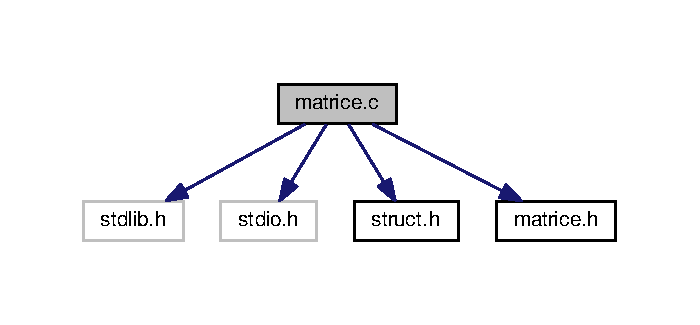
\includegraphics[width=336pt]{matrice_8c__incl}
\end{center}
\end{figure}
\subsection*{Fonctions}
\begin{DoxyCompactItemize}
\item 
int {\bfseries est\+\_\+dans\+\_\+matrice} (\hyperlink{structcaract__mat__t}{caract\+\_\+mat\+\_\+t} $\ast$cmat, int x, int y)\hypertarget{matrice_8c_a3c31a14ac91dab3b7cfc1765a5cc8509}{}\label{matrice_8c_a3c31a14ac91dab3b7cfc1765a5cc8509}

\item 
void {\bfseries creation\+\_\+matrice} (\hyperlink{structcaract__mat__t}{caract\+\_\+mat\+\_\+t} $\ast$cmat)\hypertarget{matrice_8c_ae429f6e619f7605f731f3006523d1cdb}{}\label{matrice_8c_ae429f6e619f7605f731f3006523d1cdb}

\item 
void {\bfseries init\+\_\+matrice} (\hyperlink{structcaract__mat__t}{caract\+\_\+mat\+\_\+t} $\ast$cmat)\hypertarget{matrice_8c_a2b7b061208da70a80ab7dd9f31de5c07}{}\label{matrice_8c_a2b7b061208da70a80ab7dd9f31de5c07}

\end{DoxyCompactItemize}


\subsection{Description détaillée}
Initialisation matrice. 

\begin{DoxyAuthor}{Auteur}
P\+H\+I\+L\+L\+I\+PE Marion 
\end{DoxyAuthor}
\begin{DoxyVersion}{Version}
1.\+1 
\end{DoxyVersion}
\begin{DoxyDate}{Date}
19 Mars 2018 
\end{DoxyDate}

\hypertarget{multijoueur_8c}{}\section{Référence du fichier multijoueur.\+c}
\label{multijoueur_8c}\index{multijoueur.\+c@{multijoueur.\+c}}


Fonctions outils multijoueur.  


{\ttfamily \#include $<$stdlib.\+h$>$}\\*
{\ttfamily \#include $<$stdio.\+h$>$}\\*
{\ttfamily \#include \char`\"{}struct.\+h\char`\"{}}\\*
{\ttfamily \#include \char`\"{}matrice.\+h\char`\"{}}\\*
{\ttfamily \#include \char`\"{}piege.\+h\char`\"{}}\\*
{\ttfamily \#include \char`\"{}nourriture.\+h\char`\"{}}\\*
{\ttfamily \#include \char`\"{}joueur.\+h\char`\"{}}\\*
{\ttfamily \#include \char`\"{}canard.\+h\char`\"{}}\\*
{\ttfamily \#include \char`\"{}deplacer.\+h\char`\"{}}\\*
{\ttfamily \#include \char`\"{}deplacer\+\_\+multi.\+h\char`\"{}}\\*
{\ttfamily \#include \char`\"{}labyrinthe.\+h\char`\"{}}\\*
{\ttfamily \#include \char`\"{}multijoueur.\+h\char`\"{}}\\*
Graphe des dépendances par inclusion de multijoueur.\+c\+:
% FIG 0
\subsection*{Fonctions}
\begin{DoxyCompactItemize}
\item 
\hyperlink{structjoueurm__s}{joueur\+\_\+multi\+\_\+t} \hyperlink{multijoueur_8c_a97b27c132aea39f525681767631a03a8}{joueur\+\_\+gentil} ()
\item 
\hyperlink{structjoueurm__s}{joueur\+\_\+multi\+\_\+t} \hyperlink{multijoueur_8c_a5934823e38db1e7f75825bbf0ab7b141}{joueur\+\_\+mechant} ()
\item 
void \hyperlink{multijoueur_8c_a4208d6e0692cb5efaca7d4a1c8cbabfe}{tour\+\_\+multijoueur} (\hyperlink{structcaract__mat__t}{caract\+\_\+mat\+\_\+t} $\ast$cmat, int $\ast$nourriture\+\_\+genere, int $\ast$nourriture\+\_\+accouplement, \hyperlink{structjoueurm__s}{joueur\+\_\+multi\+\_\+t} tab\mbox{[}$\,$\mbox{]}, int tour, int tampon)
\item 
int \hyperlink{multijoueur_8c_a514eac63a82d5da1b2afffa9cd49a085}{qui\+\_\+commence} (void)
\item 
void \hyperlink{multijoueur_8c_a4db4d85f20641e4a5467cff380ad88ea}{init\+\_\+tab\+\_\+joueurs} (\hyperlink{structjoueur__s}{joueur\+\_\+t} $\ast$tab, int tampon)
\begin{DoxyCompactList}\small\item\em met le nom du premier joueur a jouer en premiere place dans le tableau \end{DoxyCompactList}\item 
int \hyperlink{multijoueur_8c_ad56084052276e565587126f9cef02114}{boucle\+\_\+multi} (\hyperlink{structcaract__mat__t}{caract\+\_\+mat\+\_\+t} $\ast$cmat, \hyperlink{structjoueur__s}{joueur\+\_\+t} joueur1, \hyperlink{structjoueur__s}{joueur\+\_\+t} joueur2, int nourriture\+\_\+genere, int nourriture\+\_\+accouplement, int nb\+\_\+gen, int tampon)
\item 
int \hyperlink{multijoueur_8c_a03d2c8daaba0a3cadb621b810ee8df30}{main\+\_\+multijoueur} (\hyperlink{structcaract__mat__t}{caract\+\_\+mat\+\_\+t} $\ast$cmat, int nourriture\+\_\+genere, int nourriture\+\_\+accouplement, int nb\+\_\+gen)
\end{DoxyCompactItemize}


\subsection{Description détaillée}
Fonctions outils multijoueur. 

\begin{DoxyAuthor}{Auteur}
Maxime.\+T 
\end{DoxyAuthor}
\begin{DoxyVersion}{Version}
1.\+1 
\end{DoxyVersion}
\begin{DoxyDate}{Date}
20 fevrier 2018 
\end{DoxyDate}


\subsection{Documentation des fonctions}
\index{multijoueur.\+c@{multijoueur.\+c}!boucle\+\_\+multi@{boucle\+\_\+multi}}
\index{boucle\+\_\+multi@{boucle\+\_\+multi}!multijoueur.\+c@{multijoueur.\+c}}
\subsubsection[{\texorpdfstring{boucle\+\_\+multi(caract\+\_\+mat\+\_\+t $\ast$cmat, joueur\+\_\+t joueur1, joueur\+\_\+t joueur2, int nourriture\+\_\+genere, int nourriture\+\_\+accouplement, int nb\+\_\+gen, int tampon)}{boucle_multi(caract_mat_t *cmat, joueur_t joueur1, joueur_t joueur2, int nourriture_genere, int nourriture_accouplement, int nb_gen, int tampon)}}]{\setlength{\rightskip}{0pt plus 5cm}int boucle\+\_\+multi (
\begin{DoxyParamCaption}
\item[{{\bf caract\+\_\+mat\+\_\+t} $\ast$}]{cmat, }
\item[{{\bf joueur\+\_\+t}}]{joueur1, }
\item[{{\bf joueur\+\_\+t}}]{joueur2, }
\item[{int}]{nourriture\+\_\+genere, }
\item[{int}]{nourriture\+\_\+accouplement, }
\item[{int}]{nb\+\_\+gen, }
\item[{int}]{tampon}
\end{DoxyParamCaption}
)}\hypertarget{multijoueur_8c_ad56084052276e565587126f9cef02114}{}\label{multijoueur_8c_ad56084052276e565587126f9cef02114}
fonction qui initialise les fonctions des joueurs en mettant leur jooueur\+\_\+t passé en param, et qui fait le déroulement du jeu \index{multijoueur.\+c@{multijoueur.\+c}!init\+\_\+tab\+\_\+joueurs@{init\+\_\+tab\+\_\+joueurs}}
\index{init\+\_\+tab\+\_\+joueurs@{init\+\_\+tab\+\_\+joueurs}!multijoueur.\+c@{multijoueur.\+c}}
\subsubsection[{\texorpdfstring{init\+\_\+tab\+\_\+joueurs(joueur\+\_\+t $\ast$tab, int tampon)}{init_tab_joueurs(joueur_t *tab, int tampon)}}]{\setlength{\rightskip}{0pt plus 5cm}void init\+\_\+tab\+\_\+joueurs (
\begin{DoxyParamCaption}
\item[{{\bf joueur\+\_\+t} $\ast$}]{tab, }
\item[{int}]{tampon}
\end{DoxyParamCaption}
)}\hypertarget{multijoueur_8c_a4db4d85f20641e4a5467cff380ad88ea}{}\label{multijoueur_8c_a4db4d85f20641e4a5467cff380ad88ea}


met le nom du premier joueur a jouer en premiere place dans le tableau 


\begin{DoxyParams}{Paramètres}
{\em tab} & tableau de joueurs \\
\hline
{\em tampon} & resultat du placement \\
\hline
\end{DoxyParams}
\index{multijoueur.\+c@{multijoueur.\+c}!joueur\+\_\+gentil@{joueur\+\_\+gentil}}
\index{joueur\+\_\+gentil@{joueur\+\_\+gentil}!multijoueur.\+c@{multijoueur.\+c}}
\subsubsection[{\texorpdfstring{joueur\+\_\+gentil()}{joueur_gentil()}}]{\setlength{\rightskip}{0pt plus 5cm}{\bf joueur\+\_\+multi\+\_\+t} joueur\+\_\+gentil (
\begin{DoxyParamCaption}
{}
\end{DoxyParamCaption}
)}\hypertarget{multijoueur_8c_a97b27c132aea39f525681767631a03a8}{}\label{multijoueur_8c_a97b27c132aea39f525681767631a03a8}
initialise un joueur en joueur gentil \index{multijoueur.\+c@{multijoueur.\+c}!joueur\+\_\+mechant@{joueur\+\_\+mechant}}
\index{joueur\+\_\+mechant@{joueur\+\_\+mechant}!multijoueur.\+c@{multijoueur.\+c}}
\subsubsection[{\texorpdfstring{joueur\+\_\+mechant()}{joueur_mechant()}}]{\setlength{\rightskip}{0pt plus 5cm}{\bf joueur\+\_\+multi\+\_\+t} joueur\+\_\+mechant (
\begin{DoxyParamCaption}
{}
\end{DoxyParamCaption}
)}\hypertarget{multijoueur_8c_a5934823e38db1e7f75825bbf0ab7b141}{}\label{multijoueur_8c_a5934823e38db1e7f75825bbf0ab7b141}
initialise un joueur en tant que mechant \index{multijoueur.\+c@{multijoueur.\+c}!main\+\_\+multijoueur@{main\+\_\+multijoueur}}
\index{main\+\_\+multijoueur@{main\+\_\+multijoueur}!multijoueur.\+c@{multijoueur.\+c}}
\subsubsection[{\texorpdfstring{main\+\_\+multijoueur(caract\+\_\+mat\+\_\+t $\ast$cmat, int nourriture\+\_\+genere, int nourriture\+\_\+accouplement, int nb\+\_\+gen)}{main_multijoueur(caract_mat_t *cmat, int nourriture_genere, int nourriture_accouplement, int nb_gen)}}]{\setlength{\rightskip}{0pt plus 5cm}int main\+\_\+multijoueur (
\begin{DoxyParamCaption}
\item[{{\bf caract\+\_\+mat\+\_\+t} $\ast$}]{cmat, }
\item[{int}]{nourriture\+\_\+genere, }
\item[{int}]{nourriture\+\_\+accouplement, }
\item[{int}]{nb\+\_\+gen}
\end{DoxyParamCaption}
)}\hypertarget{multijoueur_8c_a03d2c8daaba0a3cadb621b810ee8df30}{}\label{multijoueur_8c_a03d2c8daaba0a3cadb621b810ee8df30}
fait le jeu en multi sur meme pc \index{multijoueur.\+c@{multijoueur.\+c}!qui\+\_\+commence@{qui\+\_\+commence}}
\index{qui\+\_\+commence@{qui\+\_\+commence}!multijoueur.\+c@{multijoueur.\+c}}
\subsubsection[{\texorpdfstring{qui\+\_\+commence(void)}{qui_commence(void)}}]{\setlength{\rightskip}{0pt plus 5cm}int qui\+\_\+commence (
\begin{DoxyParamCaption}
\item[{void}]{}
\end{DoxyParamCaption}
)}\hypertarget{multijoueur_8c_a514eac63a82d5da1b2afffa9cd49a085}{}\label{multijoueur_8c_a514eac63a82d5da1b2afffa9cd49a085}
demande quel joueur commence

\begin{DoxyReturn}{Renvoie}
renvoit 0 si c est le gentil et 1 si c est le mechant 
\end{DoxyReturn}
\index{multijoueur.\+c@{multijoueur.\+c}!tour\+\_\+multijoueur@{tour\+\_\+multijoueur}}
\index{tour\+\_\+multijoueur@{tour\+\_\+multijoueur}!multijoueur.\+c@{multijoueur.\+c}}
\subsubsection[{\texorpdfstring{tour\+\_\+multijoueur(caract\+\_\+mat\+\_\+t $\ast$cmat, int $\ast$nourriture\+\_\+genere, int $\ast$nourriture\+\_\+accouplement, joueur\+\_\+multi\+\_\+t tab[], int tour, int tampon)}{tour_multijoueur(caract_mat_t *cmat, int *nourriture_genere, int *nourriture_accouplement, joueur_multi_t tab[], int tour, int tampon)}}]{\setlength{\rightskip}{0pt plus 5cm}void tour\+\_\+multijoueur (
\begin{DoxyParamCaption}
\item[{{\bf caract\+\_\+mat\+\_\+t} $\ast$}]{cmat, }
\item[{int $\ast$}]{nourriture\+\_\+genere, }
\item[{int $\ast$}]{nourriture\+\_\+accouplement, }
\item[{{\bf joueur\+\_\+multi\+\_\+t}}]{tab\mbox{[}$\,$\mbox{]}, }
\item[{int}]{tour, }
\item[{int}]{tampon}
\end{DoxyParamCaption}
)}\hypertarget{multijoueur_8c_a4208d6e0692cb5efaca7d4a1c8cbabfe}{}\label{multijoueur_8c_a4208d6e0692cb5efaca7d4a1c8cbabfe}
Fonction qui defini le contenu d\textquotesingle{}un tour de jeu en multi joueur 
\hypertarget{outils_8c}{}\section{Référence du fichier outils.\+c}
\label{outils_8c}\index{outils.\+c@{outils.\+c}}


Programme comprennant les piegfes dans le laby.  


{\ttfamily \#include $<$stdlib.\+h$>$}\\*
{\ttfamily \#include $<$stdio.\+h$>$}\\*
Graphe des dépendances par inclusion de outils.\+c\+:
\nopagebreak
\begin{figure}[H]
\begin{center}
\leavevmode
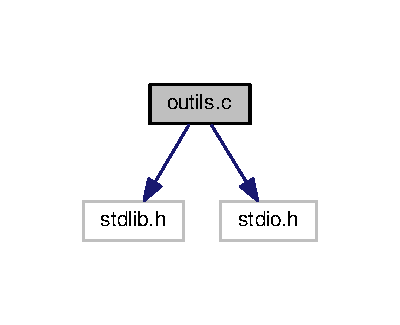
\includegraphics[width=192pt]{outils_8c__incl}
\end{center}
\end{figure}
\subsection*{Fonctions}
\begin{DoxyCompactItemize}
\item 
int {\bfseries rand\+\_\+map} (int taille\+\_\+mat)\hypertarget{outils_8c_a58eb67d99f2022d47a39898694b50ec4}{}\label{outils_8c_a58eb67d99f2022d47a39898694b50ec4}

\item 
void \hyperlink{outils_8c_aad258ae47a303ed4dbc0409fbee8ea32}{entrer\+\_\+int} (int $\ast$val)
\end{DoxyCompactItemize}


\subsection{Description détaillée}
Programme comprennant les piegfes dans le laby. 

\begin{DoxyAuthor}{Auteur}
V\+A\+I\+D\+IE Camille, T\+O\+U\+ZE Maxime,M\+A\+R\+C\+H\+A\+ND Killian,P\+H\+I\+L\+I\+P\+PE Marion 
\end{DoxyAuthor}
\begin{DoxyVersion}{Version}
1.\+0 
\end{DoxyVersion}
\begin{DoxyDate}{Date}
20 Février 2018 
\end{DoxyDate}


\subsection{Documentation des fonctions}
\index{outils.\+c@{outils.\+c}!entrer\+\_\+int@{entrer\+\_\+int}}
\index{entrer\+\_\+int@{entrer\+\_\+int}!outils.\+c@{outils.\+c}}
\subsubsection[{\texorpdfstring{entrer\+\_\+int(int $\ast$val)}{entrer_int(int *val)}}]{\setlength{\rightskip}{0pt plus 5cm}void entrer\+\_\+int (
\begin{DoxyParamCaption}
\item[{int $\ast$}]{val}
\end{DoxyParamCaption}
)}\hypertarget{outils_8c_aad258ae47a303ed4dbc0409fbee8ea32}{}\label{outils_8c_aad258ae47a303ed4dbc0409fbee8ea32}
Permet une entrée d\textquotesingle{}un int, et seulement un int


\begin{DoxyParams}{Paramètres}
{\em val} & fonctionne comme un scanf sans le cham \% \\
\hline
\end{DoxyParams}

\hypertarget{piege_8c}{}\section{Référence du fichier piege.\+c}
\label{piege_8c}\index{piege.\+c@{piege.\+c}}


Programme comprennant les pieges dans le laby.  


{\ttfamily \#include $<$stdlib.\+h$>$}\\*
{\ttfamily \#include $<$stdio.\+h$>$}\\*
{\ttfamily \#include \char`\"{}struct.\+h\char`\"{}}\\*
{\ttfamily \#include \char`\"{}matrice.\+h\char`\"{}}\\*
Graphe des dépendances par inclusion de piege.\+c\+:\nopagebreak
\begin{figure}[H]
\begin{center}
\leavevmode
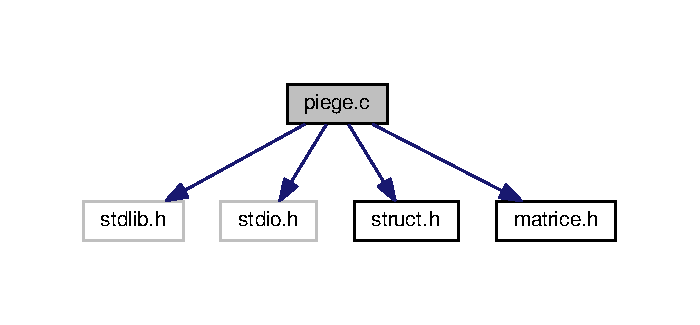
\includegraphics[width=336pt]{piege_8c__incl}
\end{center}
\end{figure}
\subsection*{Fonctions}
\begin{DoxyCompactItemize}
\item 
void {\bfseries piege} (\hyperlink{structcaract__mat__t}{caract\+\_\+mat\+\_\+t} $\ast$cmat)\hypertarget{piege_8c_aa15334529c17f0361233d2032aab58d4}{}\label{piege_8c_aa15334529c17f0361233d2032aab58d4}

\item 
void {\bfseries presence\+\_\+piege} (\hyperlink{structcaract__mat__t}{caract\+\_\+mat\+\_\+t} $\ast$cmat)\hypertarget{piege_8c_a9dcbf50e93fc3e9879dfc4d78a676b2f}{}\label{piege_8c_a9dcbf50e93fc3e9879dfc4d78a676b2f}

\end{DoxyCompactItemize}


\subsection{Description détaillée}
Programme comprennant les pieges dans le laby. 

\begin{DoxyAuthor}{Auteur}
V\+A\+I\+D\+IE Camille 
\end{DoxyAuthor}
\begin{DoxyVersion}{Version}
1.\+0 
\end{DoxyVersion}
\begin{DoxyDate}{Date}
20 Février 2018 
\end{DoxyDate}

\hypertarget{reproduction_8c}{}\section{Référence du fichier reproduction.\+c}
\label{reproduction_8c}\index{reproduction.\+c@{reproduction.\+c}}


Programme comprennant la reproduction des canards.  


{\ttfamily \#include \char`\"{}struct.\+h\char`\"{}}\\*
{\ttfamily \#include \char`\"{}matrice.\+h\char`\"{}}\\*
{\ttfamily \#include \char`\"{}joueur.\+h\char`\"{}}\\*
{\ttfamily \#include $<$stdio.\+h$>$}\\*
{\ttfamily \#include $<$stdlib.\+h$>$}\\*
Graphe des dépendances par inclusion de reproduction.\+c\+:
\nopagebreak
\begin{figure}[H]
\begin{center}
\leavevmode
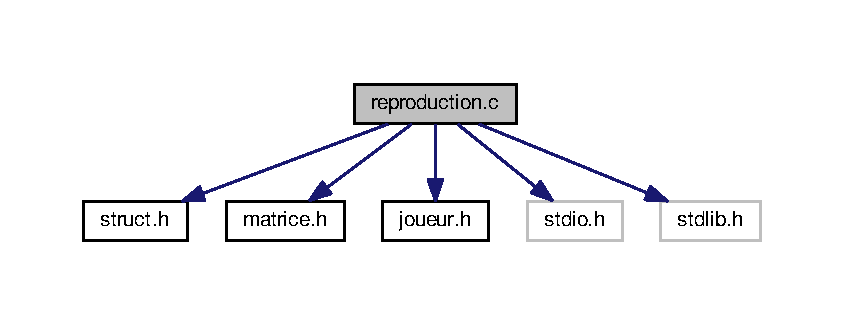
\includegraphics[width=350pt]{reproduction_8c__incl}
\end{center}
\end{figure}
\subsection*{Fonctions}
\begin{DoxyCompactItemize}
\item 
int {\bfseries ou\+\_\+pondre} (\hyperlink{structcaract__mat__t}{caract\+\_\+mat\+\_\+t} $\ast$cmat, int $\ast$i, int $\ast$j)\hypertarget{reproduction_8c_ac26b148d861ba7701a8b52548640a277}{}\label{reproduction_8c_ac26b148d861ba7701a8b52548640a277}

\item 
void {\bfseries reproduction} (\hyperlink{structcaract__mat__t}{caract\+\_\+mat\+\_\+t} $\ast$mat, int nourriture\+\_\+accouplement, \hyperlink{structjoueur__s}{joueur\+\_\+t} joueur, \hyperlink{structjoueur__s}{joueur\+\_\+t} joueur2)\hypertarget{reproduction_8c_acbf5003c554076aa8570fb76e24122ca}{}\label{reproduction_8c_acbf5003c554076aa8570fb76e24122ca}

\end{DoxyCompactItemize}


\subsection{Description détaillée}
Programme comprennant la reproduction des canards. 

\begin{DoxyAuthor}{Auteur}
V\+A\+I\+D\+IE Camille 
\end{DoxyAuthor}
\begin{DoxyVersion}{Version}
1.\+0 
\end{DoxyVersion}
\begin{DoxyDate}{Date}
20 Février 2018 
\end{DoxyDate}

%--- End generated contents ---

% Index
\backmatter
\newpage
\phantomsection
\clearemptydoublepage
\addcontentsline{toc}{chapter}{Index}
\printindex

\end{document}
